
\documentclass[12pt,a4paper,final]{article}
\usepackage[utf8]{inputenc}
\usepackage[francais]{babel}
\usepackage[T1]{fontenc}
\usepackage{amsmath}
\usepackage{amsfonts}
\usepackage{amsthm}
\usepackage{color}
\usepackage{amssymb}
\usepackage{graphicx}
\usepackage{algorithm}
\usepackage{algorithmic}
\usepackage{fancyhdr}
\usepackage[fs]{umons-coverpage}
\usepackage{hyperref}


%%###### START CHANGE HERE ######
\author{S. Opsommer \& R. Cambier}
\title{Rapport du projet Pac-Man}
\umonsAuthor{\begin{tabular}{lll}
\textsc{Cambier} & Robin & ROBIN.CAMBIERR@student.umons.ac.be\\
\textsc{Opsommer} & Sophie & SOPHIE.OPSOMMER@student.umons.ac.be\\
\end{tabular} }
%% The main title of your thesis
\umonsTitle{Rapport du projet Pac-Man}
%% The sub-title of your thesis
\umonsSubtitle{Projet réalisé dans le cadre \\de la 1ère Master en Sciences Informatiques \\pour le cours de \og Software Evolution \fg}
%% Your supervisor(s)
\umonsSupervisor{\begin{tabular}{ll}
\textit{Titulaire} : & T. \textsc{Mens} \\
\textit{Assistant} : & M. \textsc{Claes} \\
\end{tabular}}
%% The date (or academic year)
\umonsDate {\hfill Ann\'ee Acad\'emique 2014-2015}
%%###### END CHANGEMENT ######

\newcommand{\smalltitle}[1]{\bigskip\large\textbf{#1}\par\normalsize\medskip}
\newcommand{\partitle}[1]{\bigskip\textit{\underline{#1}}\par\medskip}
\newcommand{\annexe}[1]{annexe~\ref{#1} (page~\pageref{#1})}
\newcommand{\labelfigure}[1]{figure~\ref{#1} (page~\pageref{#1})}

\graphicspath{{images/}}

\newtheorem{defi}{Définition}
%\newtheorem{note}{Note}
%\newtheorem{prop}{Propriété}
%\newtheorem{exemple}{Exemple}
%\newtheorem{corollaire}{Corollaire}
%\newtheorem{lemme}{Lemme}
%\newtheorem{rem}{Remarque}
%\newtheorem{thm}{Théorème}

\fancyhf{}
\chead{\leftmark}
\rfoot{\thepage}

\begin{document}
\umonsCoverPage
\pagebreak
\pagestyle{fancy}
%%%%%%%%%%%%%%%%%%%%%%%%%%%%%%%%%%%%%%%%%%%%%%%%%%%%%%%%%%%%%%%%%%%%%%%%%%%%%%%%%%%%%%%
\newpage
\thispagestyle{empty}
\vspace*{\stretch{1}}
\begin{abstract}
\addcontentsline{toc}{section}{Résumé}
Ce \emph{rapport} est rendu dans le cadre du cursus de première année de \og Master en Sciences Informatiques\fg  pour le cours de \emph{Software Evolution} (dont le titulaire est Mr. \emph{T. Mens} et l'assistant est Mr. \emph{M. Claes} en année académique 2014-2015) . Le but de ce rapport est de présenter les résultats de la réalisation du projet Pac-Man.
\end{abstract}
\vspace*{\stretch{1}}

%----------------------------------------------------------------------------------------
%	Acknoledge
%----------------------------------------------------------------------------------------
%%%%%remerciements%%%%%% bon example dans le livre de référence musimoti
%\pagenumbering{gobble}
%\clearpage
%\thispagestyle{empty}
%Note aux lecteurs : 
%Cette version n'a pas été relue et donc comporte probablement beaucoup de fautes d'orthographes. une version corrigée est postée sur moodle.
%Merci de votre compréhension
%Sophie
%\clearpage

%----------------------------------------------------------------------------------------
%	TABLE OF CONTENTS
%----------------------------------------------------------------------------------------
\newpage
\thispagestyle{empty}
\tableofcontents
%%%%%%%%%%%%%%%%%%%%%%%%%%%%%%%%%%%%%%%%%%%%%%%%%%%%%%%%%%%%%%%%%%%%%%%%%%%%%%%%%%%%%%%%
%%###### LE RAPPORT COMMENCE ICI ######
\newpage
\section{Introduction}\label{sec:intro}
\subsection{Problème posé}
A partir d'un code existant, ce projet consiste à : 
\begin{itemize}
\item analyser la qualité du logiciel, en utilisant des techniques d'analyse statique du code (par exemple, la détection du code dupliqué et des bad smells, les diverses métriques de qualité) et les outils d'analyse dynamique du code (par exemple, le profilage, la couverture du code et des tests);
\item améliorer la qualité et la structure du code (en utilisant des refactorings, en introduisant des design patterns, et en modularisant le code) ;
\item étendre le logiciel avec de nouvelles fonctionnalités (évolution), et étudier l'effet de cela sur la qualité du code;
\item tester le logiciel avant et après chaque modification. Ceci implique que vous devez ajouter des tests unitaires (unit tests) pour au moins les fragments du code modifiés ou ajoutés, et d'appliquer des tests de régression à chaque modification.
\end{itemize}

\subsection{Etapes clés}
Les étapes clés du projet sont les suivantes : (chronologiquement)
\begin{enumerate}
\item Analyse de la qualité de la premiére version du code (section \ref{sec:etape1})
\item Ajout de tests unitaires à la première version du code (section \ref{sec:etape2}), et vérification de la couverture des tests
\item Refactoring du code pour en améliorer la qualité et la structure (section \ref{sec:etape3})
\item Analyse des améliorations de qualité et tests de régression (section \ref{sec:etape4})
\item Extension du logiciel et ajout des tests unitaires pour cette extension (section \ref{sec:etape5})
\item Analyse de la qualité de cette extension et tests de régression (section \ref{sec:etape6})
\item Etude de l'historique de la qualité logicielle entre toutes les versions du code (section \ref{sec:etape7})
\end{enumerate}
%%%%%%%%%%%%%%%%%%%%%%%%%%%%%%%%%%%%%%%%%%%%%%%%%%%%%%%%%%%%%%%%%%%%%%%%%%%%%%%%%%
\section{Etape 1 : Première analyse de la qualité du logiciel}\label{sec:etape1}
Avant toute modification, il convient d'analyser l'état de la qualité du logiciel afin de se rendre compte des améliorations à effectuer, des corrections à appliquer si des mauvaises pratiques sont observées. Cette analyse se fera à l'aide d'outils d'analyse de code tel que les IDE\footnote{IDE : Integrated Development Environment (Environnement de développement).} Eclipse\footnote{Eclipse : \url{https://eclipse.org/} version : Eclipse Luna SR2 (4.4.2).} et IntelijIdea\footnote{InteligIdea : \url{https://www.jetbrains.com/idea} version : Community Edition 14.0.3 } et les programmes CodePro\footnote{CodePro : \url{https://marketplace.eclipse.org/content/codepro-analytix} version : CodePro Analytix 7.1.0.r37}, InCode\footnote{InCode : \url{https://marketplace.eclipse.org/content/incode-helium} version 2.0.1} et VisualVM\footnote{VisualVM : \url{http://visualvm.java.net/} version 1.3.8}.

\subsection{Enoncé}
Le but de la première étape clé est d'analyser la qualité du logiciel pour avoir une première idée de ce qu'il faudra corriger si l'on désire améliorer la qualité. Cette première analyse est également l'occasion de comprendre l'architecture et la dynamique du système.
Pour cette étape clé il est demandé de :
\begin{enumerate}
%\item Calculer la valeur de plusieurs métriques logicielles permettant d'estimer la qualité du logiciel, d'interpréter les résultats des métriques, et de mettre en évidence les modules (packages, classes ou méthodes) qui devraient être traités prioritairement afin d'améliorer leur qualité ainsi que la raison pour laquelle ils sont prioritaires.
\item Déterminer les classes et les méthodes qui sont couvertes par des tests unitaires, et mettre en évidence les méthodes pour lesquelles de nouveaux tests unitaires devraient être créés prioritairement.
%\item Répertorier les portions de code qui ne sont pas utilisées et qui pourraient donc être supprimées sans altérer le comportement du système.
%\item Répertorier les portions de code qui sont redondantes (code dupliqué) et qui pourraient donc être éliminées par une restructuration du système sans altérer son comportement.
%\item Détecter la présence de bad smells. En trouvez-vous une plus forte concentration dans certains modules ?
\item Analyser les performances du système en terme d'utilisation CPU et de consommation de mémoire. Repérez les parties du code créant un goulot d'étranglement et précisez les modules qui devraient être retravaillés afin de procéder à un déoulottage du système.
\end{enumerate}
%TODO :    %Performances			%Antipattern		%Test		%Profilage
Décrivez la qualité globale du système. Quel serait, selon vous, le coût nécessaire à sa maintenance et à son évolution ?
%%%%%%%%%%%%%%%%%%%%%%%%%%%%%%%%%%%%%%%%%%%%%%%%%%%%%
\subsection{Résultat}

\subsubsection{Code dupliqué}\label{codeduplique}
Du code dupliqué consiste à trouver au sein d'un projet des blocs de lignes de code identique en plusieurs exemplaires.
C'est un facteur de mauvaise qualité parce que ça rend le code plus difficile à changer, à maintenir, à comprendre,...\\
Les solutiuons qui sont offertent par les languages de programmation sont les méthodes, les fonctions, les librairies, l'encapsulation des objets. Eviter de dupliquer du code permet d'avoir un programme plus cohésif.
\begin{figure}[!h]
	\centering
	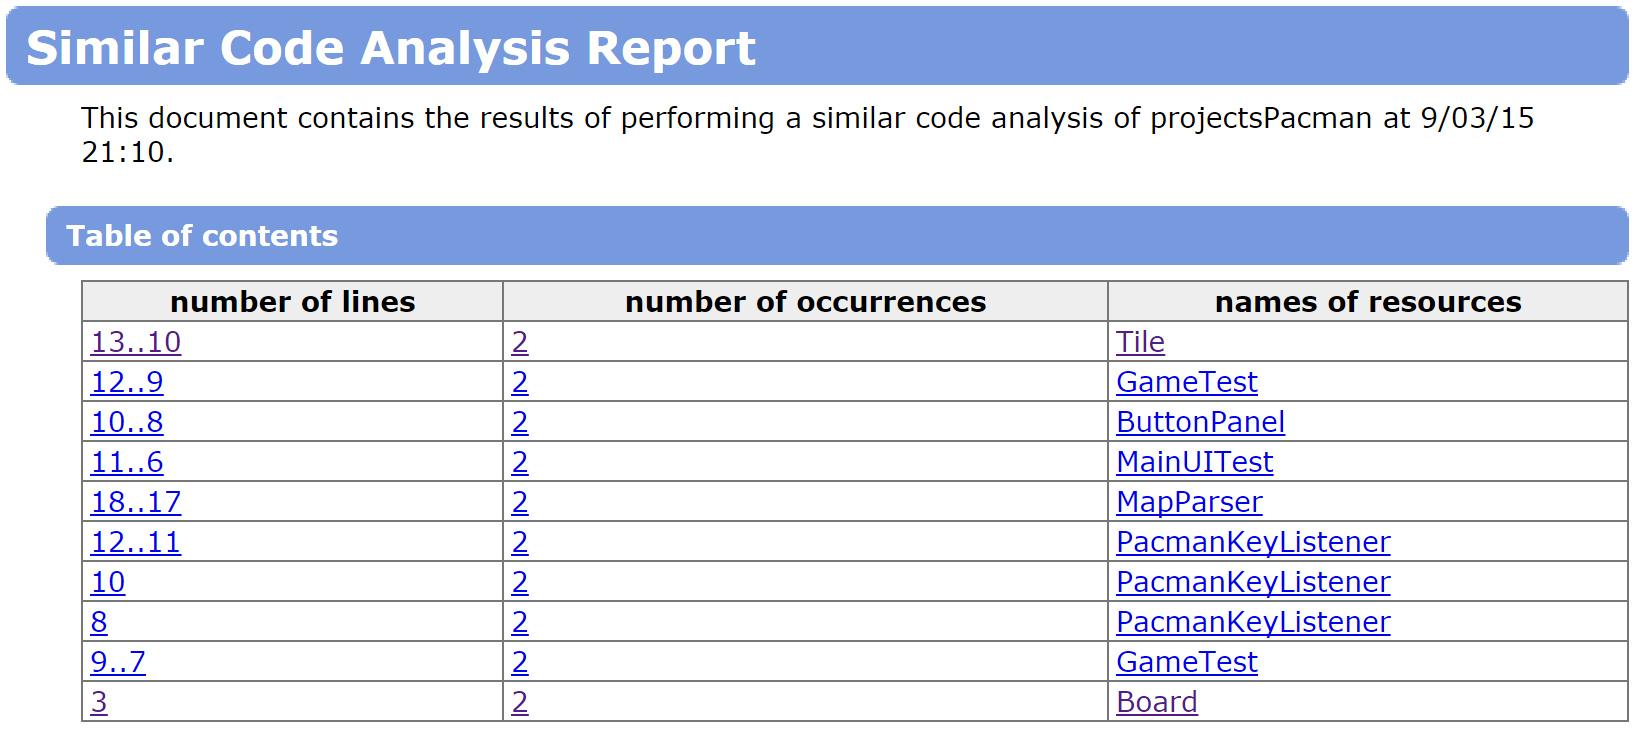
\includegraphics[width=\textwidth]{SimilarCode_00.png}
	\caption{\label{SimilarCode0}Résultat de l'analyse de "code dupliqué" par CodePro}
\end{figure}
Pour analyser cette métrique, nous avons utiliser le programme CodePro à partir de l'interface d'Eclipse ( Eclipse -> CodePro Tools -> Find Similar Code).\\
Nous pouvons observer sur la \labelfigure{SimilarCode0} que cet outils a détécté 10 blocs de code. Les figures de l'\annexe{SimilarCode} permettent de visualiser les différents blocs de code.
Les classes concernées sont : Tile.java, GameTest.java, ButtonPanel.java, MainUITest.java, MapParser.java, PacmanKeyListener.java, PacmanKeyListener.java, PacmanKeyListener.java,  GameTest.java, Board.java.\\
Ce résultat n'est pas bon, mais on peut observer que les blocs se trouve chaque fois dans une même classe. Il sera donc probablement possible de créer des fonction pour chacun de ses cas.



\subsubsection{Dépendences cycliques}\label{dépendances}
Une dépendance cyclique peut-être appelée dépendance cyclique directe ou indirecte et elle a la même difinition qu'il s'agisse de dépendances entre des projets, entre des packages ou entre des classes. Quand on a une dépendance directe, on a un élément X qui dépend d’un élément Y qui dépend lui-même de X. Contrairement à la dépendance cyclique indirecte où la situation dans laquelle on se trouve est tel que X dépend de Y, Y dépend de Z et Z dépend de X.
Du point de vue de la compilation, plus une dépendance est haut niveau, plus elle est à traiter en priorité. En effet entre deux classes, ce n'est pas très grave et ça ne pose généralement pas de problème. Entre deux package c'est fortement déconseillé même s'il est généralement possible de compiler le projet. Par contre entre deux projets, l'issue est fatale puisque chaque projet doit-être compilé avant de pouvoir compiler l'autre.\\
Du point de vue de la maintenance, une dépendance d'un élément A à un élément B et vice-versa impose que pour pouvoir modifier A, il faut commencer par modifier B et pour pouvoir modifier B, il faut commencer par retravailler B. L'évolution de ses éléments est donc compliquée.\\
Pour pallier à ce genre de problème, plusieurs pistes sont possible : déplacer les éléments (les classes si le problème concerne deux packages ou la(les) méthodes si le soucis se situe entre deux classes), redécouper certaines éléments (pour mieux associer les blocs de code aux éléments qui en ont besoin), regrouper les éléments (pour n'en former plus qu'un seul),... %piste de solution à l'adresse  :http://blog.developpez.com/wichtounet/p8723/jtheque/osgi_et_dependances_cycliques
\begin{figure}[!h]
	\centering
	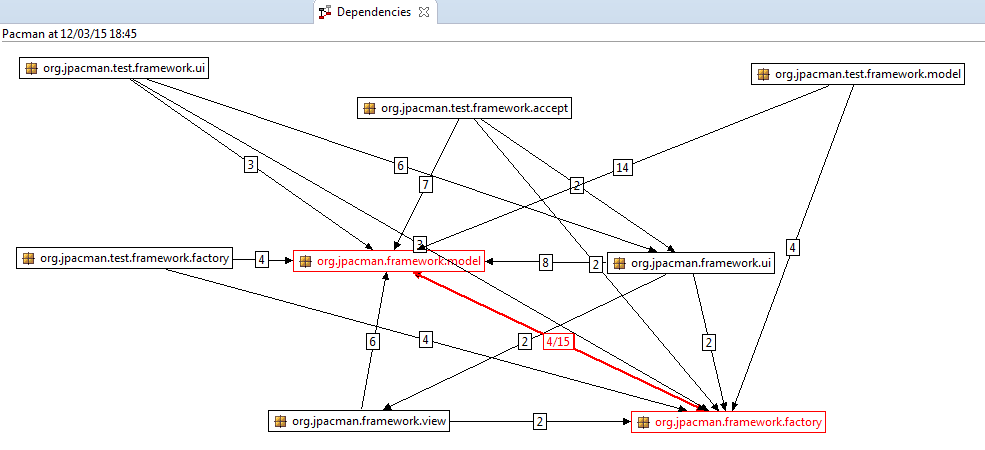
\includegraphics[width=\textwidth]{DependenciesPackages.png}
	\caption{\label{dependenciesPackage}Détail de l'analyse des dépendences cycliques des packages du projet.}
\end{figure}
\begin{figure}[!h]
	\centering
	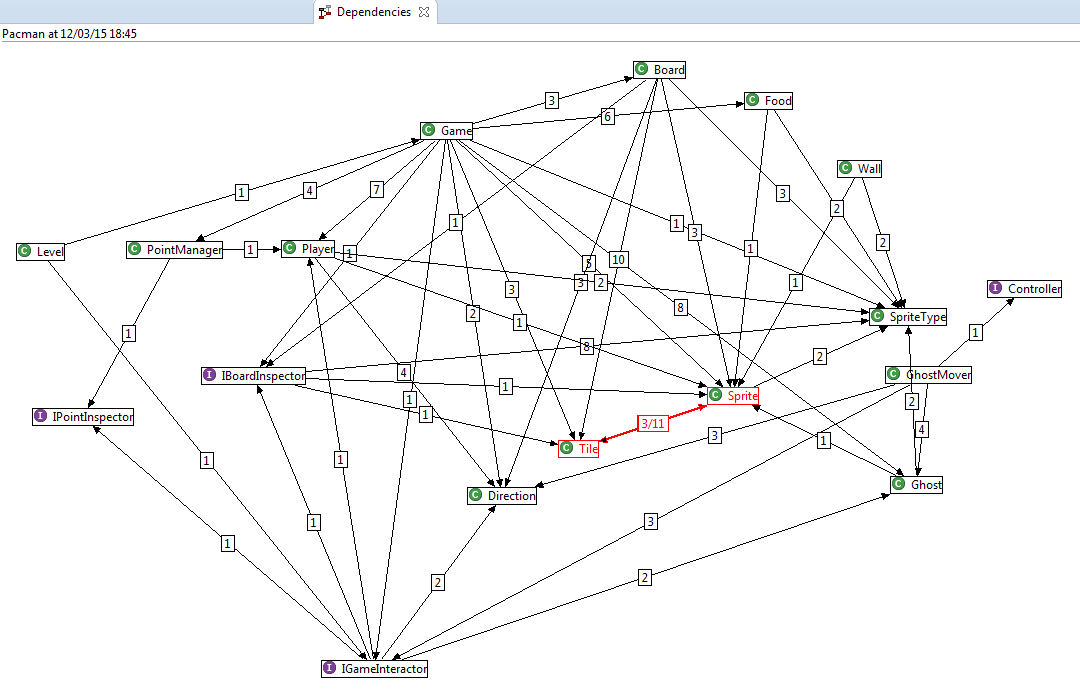
\includegraphics[width=\textwidth]{DependenciesModel.png}
	\caption{\label{dependenciesModel}Détail de l'analyse des dépendences cycliques du package Model.}
\end{figure}
Cet métrique a aussi été visualisée à partir de l'outil CodePro depuis Eclipse (Eclipse -> CodePro Tools -> Analyse Dependencies).
On peut observer sur la \labelfigure{dependenciesPackage} et la \labelfigure{dependenciesModel} qu'il existe des dépendences cycliques au sein du package Model (entre les classes Sprite et Tile) et entre le package Model et le package Factory.\\
L'\annexe{Dependencies} contient toutes les autres visualisations qui n'ont pass révélé de problème de dépendances.


\subsubsection{Code inutile}\label{deadCode}
Du code inutile, aussi appelé "Dead Code", correspond à des lignes de code qui sont compilée mais qui ne sont jamais utilisée. 
C'est fréquement du code qui a été utile à une fonctionnalité et lorsque cette fonctionnalité à été supprimée/ réécrite, déplacée,... ce code est resté. Le problème dans ce cas est que ça ralentit la compréhension du développeur lors de la lecture, ça gaspille des ressources au compilateur et lors de l'éxécution.\\
La solution est généralement de supprimer ses lignes de code.
\begin{figure}[!h]
	\centering
	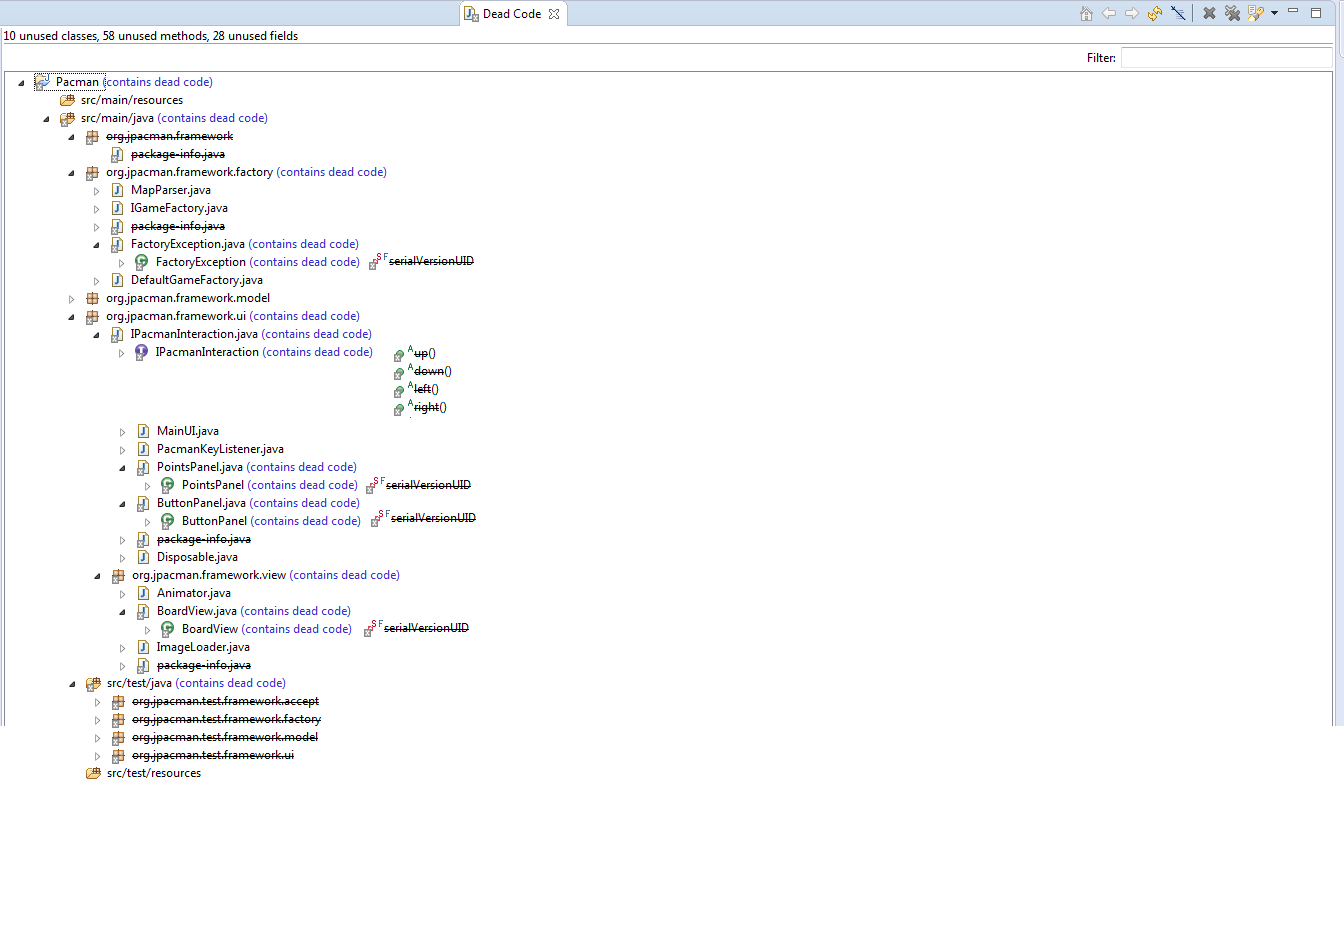
\includegraphics[width=\textwidth]{DeadCode.png}
	\caption{\label{deadcode}Détail de l'analyse des parties de code non utilisé lors de l'éxécution du programme.}
\end{figure}
L'outil utilisé reste CodePro depuis Eclipse (Eclipse -> CodePro Tools -> Find dead code).\\
Attention tout de même à ne pas tout supprimer sans réfléchir, en effet, on observer sur la \labelfigure{deadcode} que les packages contenant les test sont considéré comme inutile. Ils le sont en effet lors de l'éxécution du programme, mais ne le sont pas au bon développement du programme. Il en va de même pour les variables "serialVersionUID". Ces variables, bien que inutile lors de l'exécution, doivent-être présente dans les classes qui étendent (directement ou indirectement) la classe "Sérializable". Leur valeur est indispensable pour des applications qui transittent par le réseau mais leur existence ne peut causer aucun tort. Pour ce qui est des fichiers "package-info.java", il sont a nouveau inutule lors de l'exécution du code, mais permettent de contenir les commentaires contenant l'information relative au package en vue de la création de la javadoc. Ces fichiers sont donc à conserver (et à complêter dans certains cas).\\
L'analyse a aussi été effectuée par l'outil Code Inspector de IntelijIdea et donne d'autres résultats complémentaires. Ceux font référence à des méthodes complètes qui ne sont jamais appelées.\\
La solution la plus rapide, est simplement de supprimer ses méthodes. Seulement si lors d'une future amélioration, on se rend compte qu'elles auraient pu être nécessaire, on doit recommencer le travail. Une autre solution pourrait-être de mettres ces fonctions en commentaire afin de ne pas devoir réécrire ces fonctions.\\
Les modifications à éffectuées, bien que nombreuses, sont donc mineures.


\subsubsection{Javadoc}\label{javadoc}
La javadoc est une documentation standard au format HTML pour les programmes developpé en JAVA. Elle est créée de façon automatique par la plupart des outils de développement en se basant sur les tags placés dans le code au dessus de la déclaration de chaque classe et de chaque méthode (pour la documentation des packages, elle se trouve dans les fichiers "paquage-info.java").
L'utiliser est un plus mais ne consiste en rien en une obligation (mais alors il sera tout de même fortement conseillé d'utiliser les commentaires classique pour constituer un code suffisemment documenter à la compréhension).\\
Grace à l'outil CodePro d'Eclipse, il a été observé (non illustré parce que toutes les classes sont a revoir) que en règle générale, les classes sont documentée. L'outil détecte bien quelques manquement, mais ce sont généralement l'un ou l'autre tag qu'il détecte manquant mais qui ne perturbe pas la compréhension ainsi que les classes DefaultGameFactory, Game, IBoardInspector, IPointInspector, Player et PointManager dont les méthodes ne sont pas commentée et les méthodes issues d'une interface (sous l'annotation "@Overhide").
%Code inspector de Intelijidea a repérer le tag @param sprite manquant à la ligne 233 de la fonction spriteImage(Sprite) de la calsse BoardVieuw du package org.jpacman.framework.view


\subsubsection{Test unitaire}
Cet analyse sera détaillée dans la section suivante \ref{sec:etape2}.


\subsubsection{Flux de conception}
A l'aide de l'outil InCode intégré à Eclipse, on peut entre-autre observer la conception du programme sur la \labelfigure{designflaws} dont la légende se trouve à l'\annexe{designflawsLeg}
\begin{figure}[!h]
	\centering
	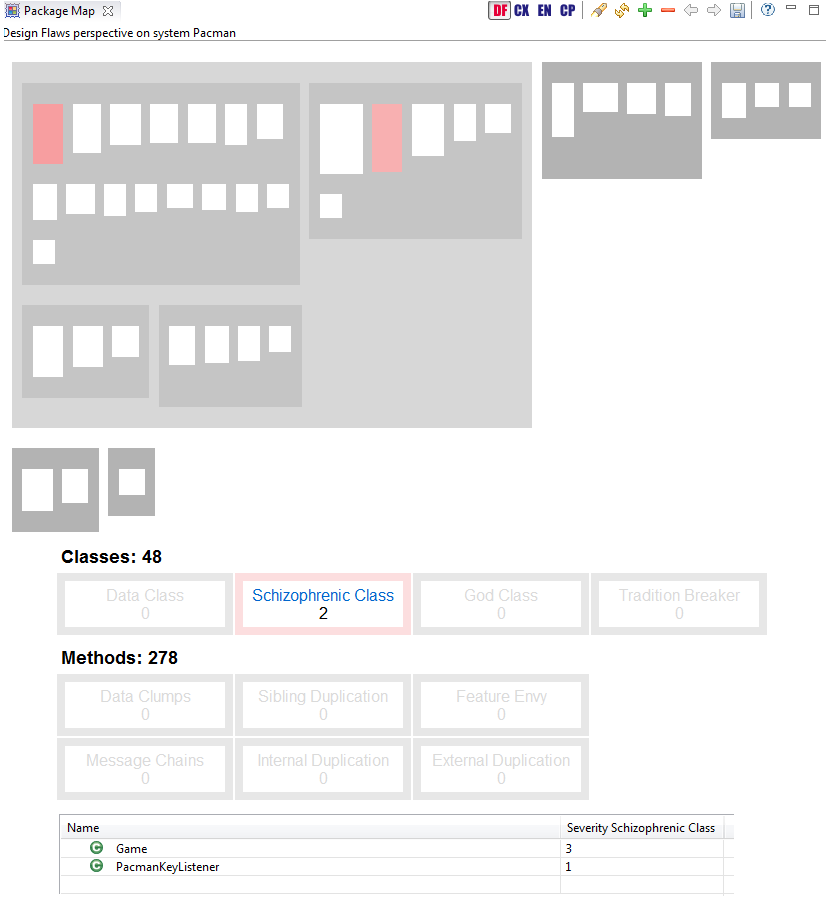
\includegraphics[width=\textwidth]{InCodeDesignFlaws.png}
	\caption{\label{designflaws}Analyse de la conception du programme (sa structure) par InCode.}
\end{figure}
La \labelfigure{designflaws} illistre donc que Il n'y a pas de gros problèmes dans l'application(point de vue structure) cependant 2 classes ont tout de même un comportement inadéquat : Game et PacmanKeyListener. Ils sont répertoriées comme des classes schizophréniques.\\
Ces classes ont la particularité  d'être utilisée par des groupes disjoints de classes de clients utilisant des fragments disjoints de la classe.\\
Plusieurs solution sont possible pour résoudre ce genre de problème :
\begin{itemize}
\item Regrouper les éléments qui sont utilisé par des groupe disjoints de clients et en faire 2 classes distincte.
\item Revoir l'accessibilité des éléments qui la contiennent.
\item Regardez 'aperçu de la vue "couplage" pour identifier toutes les dépendances basée sur les appels entre la classe et des classes externes.
\end{itemize}


\subsubsection{Complexité}
A l'aide de l'outil InCode intégré à Eclipse, on peut entre-autre observer la complexité de l'application sur la \labelfigure{complexity} dont le détail de la légende se trouve à l'\annexe{complexityLeg}
\begin{figure}[!h]
	\centering
	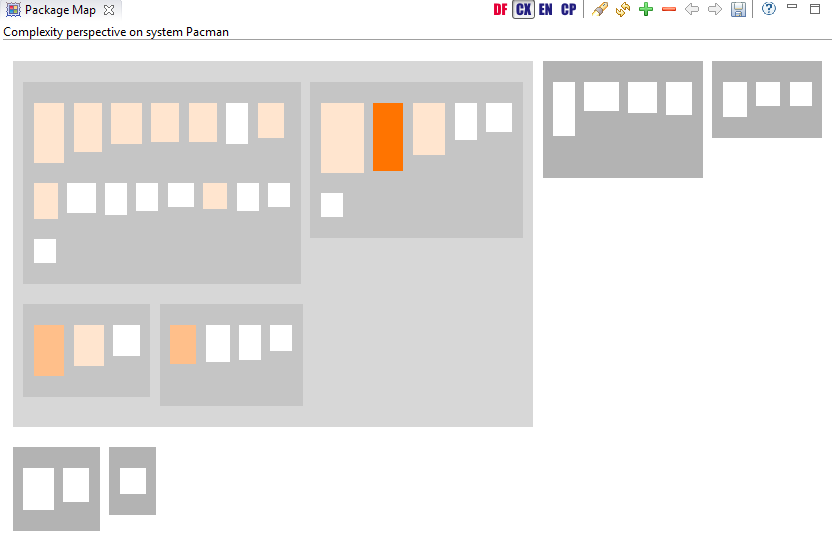
\includegraphics[width=\textwidth]{InCodeComplexity.png}
	\caption{\label{complexity}Analyse de la complexité par InCode.}
\end{figure}
Cette figure met en avant la classe PacmanKeyListener qui encourt la plus forte complexité et met un attention sur les classes BoardView et MapParser (à cause de leur grand nombre d'attributs).


\subsubsection{Encapsulation}
A l'aide de l'outil InCode intégré à Eclipse, on peut entre-autre observer la complexité de l'application sur la \labelfigure{encapsulation} dont le détail de la légende se trouve à l'\annexe{encapsulationLeg}
\begin{figure}[!h]
	\centering
	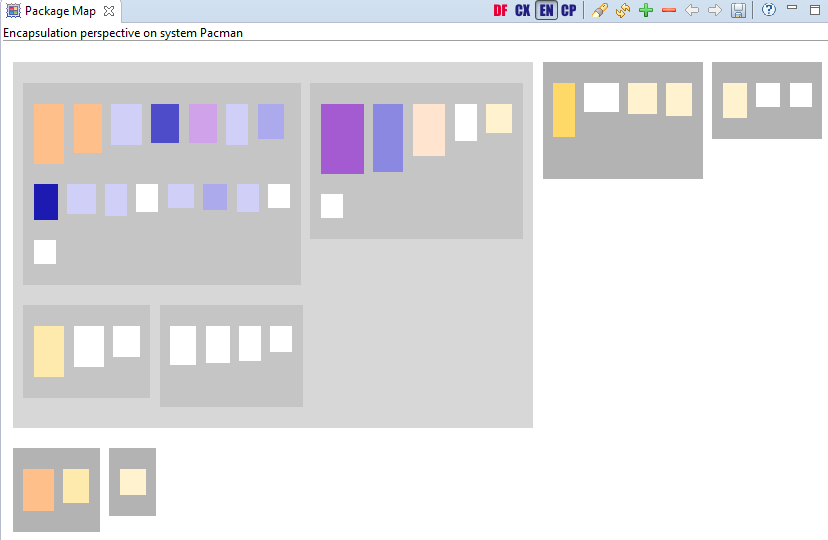
\includegraphics[width=\textwidth]{InCodeEncapsulation.png}
	\caption{\label{encapsulation}Analyse de la complexité par InCode.}
\end{figure}
Cette figuer contient beaucoup d'information, nous en retiendrons quelques unes : 
\begin{itemize}
\item La classe "MainUI" a beaucoup de clients (c'est-à-dire beaucoup d'autres classes qui accèdent aux données publiques de cette classes) dont les principaux sont "PacmanKeyListener" et "IGameInteractor". On ne sait rien concernant le nombre de fournisseurs\footnote{>provider} (c'est-à-dire beaucoup de données publiques d'autres classes auxquelles celle-ci accède) sauf qu'il est inférieur au nombre de clients.
\item La classe "Player" n'a aucun fournisseur et a beaucoup de clients dont les principaux sont "Game" et "BoardView".
\item La classe "Sprite" n'a aucun fournisseur et a beaucoup de clients dont les principaux sont "Game", "Board" et "Tile".
\item Les classes telles que "Ghost", "Controller", "Wall", "ImageLoader", "Animator", "MapParser", "IGameFactory", "FactoryException", "IPacmanInteraction" et "Disposable" n'ont ni clients ni fournisseurs.
\end{itemize}


\subsubsection{Couplage}
A l'aide de l'outil InCode intégré à Eclipse, on peut entre-autre observer la complexité de l'application sur la \labelfigure{coupling} dont le détail de la légende se trouve à l'\annexe{couplingLeg}
\begin{figure}[!h]
	\centering
	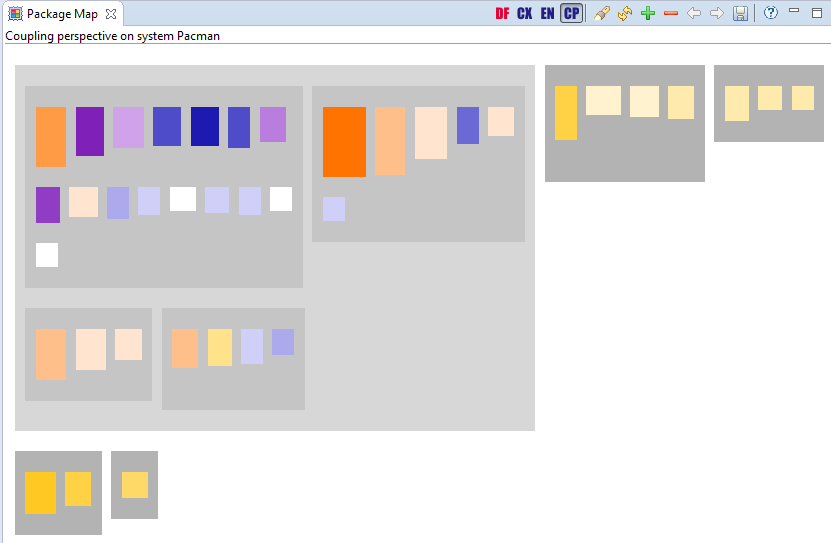
\includegraphics[width=\textwidth]{InCodeCoupling.png}
	\caption{\label{coupling}Analyse de la complexité par InCode.}
\end{figure}
Cette figuer contient aussi beaucoup d'information, nous en retiendrons quelques unes : 
\begin {itemize}
\item La classe "MainUI" a beaucoup de fournisseurs\footnote{>provider} (c'est-à-dire beaucoup de méthodes publiques d'autres classes auxquelles celle-ci accède) dont les principaux sont "GhostMover", "IGameInteractor", "Level", "BoardView", "Animator", "PacmanKeyListener", "ButtonPanel" et "PointsPanel". On ne sait rien concernant le nombre de clients (c'est-à-dire beaucoup d'autres classes qui accèdent aux méthodes publiques de cette classes) sauf qu'il est inférieur au nombre de clients.
\item La classe "Tile" a aucun fournisseur et beaucoup de client dont les principaux sont "Game", "Board" et "Sprite".
\item La classe "Board" a beaucoup de clients dont les principaux sont "Game", "MapParser" et "DefaultGameFactory". On ne sait rien concernant le nombre de fournisseurs sauf qu'il est inférieur au nombre de clients et que les principaux sont "Sprite" et "Tile".
\end{itemize}


\subsubsection{Pyramide des métriques}
A l'aide de l'outil InCode intégré à Eclipse, on peut entre-autre observer les valeurs de l'application sur la \labelfigure{pyramid} dont le détail de la légende se trouve à l'\annexe{pyramidLeg}.
\begin{figure}[!h]
	\centering
	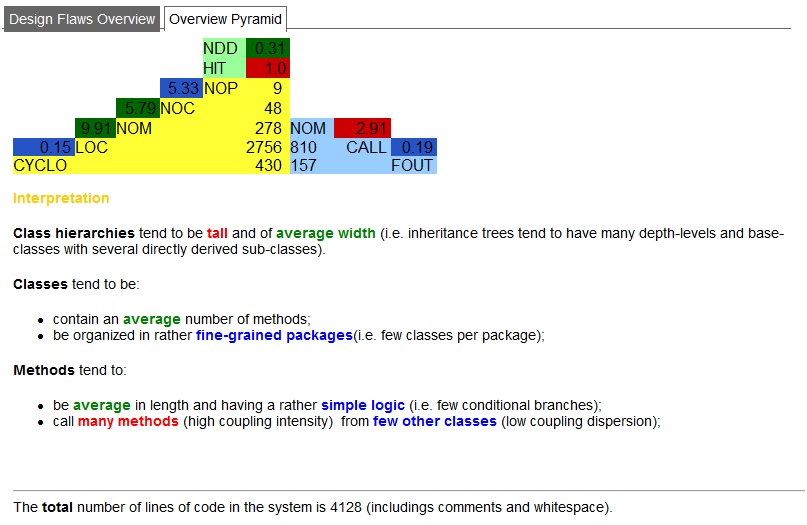
\includegraphics[width=\textwidth]{InCodePyramid.png}
	\caption{\label{pyramid}Pyramide des valeurs calculée par InCode.}
\end{figure}
Comme le précise l'interprétation de la \labelfigure{pyramid}, L'arbre que constitue les classe est grand et large.\\
Les classes ont tendance à contenir un nombre moyen de méthodes et à être organisés avec quelques classes par paquet.\\
Les méthodes tendent à être longue et avec une logique assez simple et à appeler de nombreuses méthodes (à forte intensité de couplage) de quelques autres classes (à faible dispersion de couplage).


\clearpage
\subsubsection{Métriques}
Grace à l'outil de calcul des métriques d'Eclipse, on peut observer les résulats présent à la \labelfigure{métrique0}, la \labelfigure{métrique1} et la \labelfigure{métrique2}. 
\begin{figure}[!h]
	\centering
	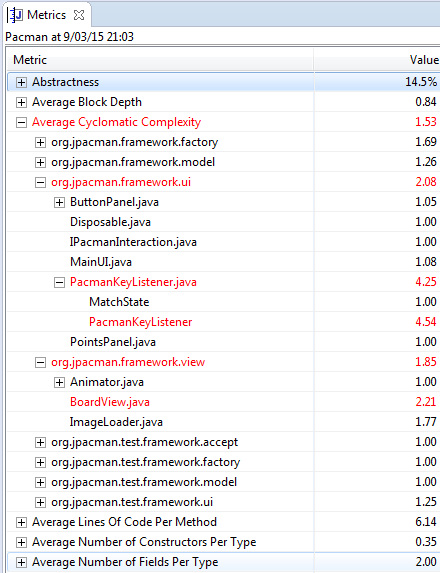
\includegraphics[height=\textheight]{Metrique0.png}
	\caption{\label{métrique0}Détails de l'analyse des métriques du projet (partie 1).}
\end{figure}

\smalltitle{Complexité cyclique moyenne}
Il s'agit de la moyenne de la complexité cyclomatique de chacune des méthodes. La complexité cyclomatique d'une méthode unique est une mesure du nombre de chemins distincts de l'exécution dans le procédé. Elle est mesurée par l'ajout d'une voie pour la méthode avec chacun des chemins créés par des instructions conditionnelles (telles que "if" et "for") et les opérateurs (tels que "? :").
\begin{figure}[!h]
	\centering
	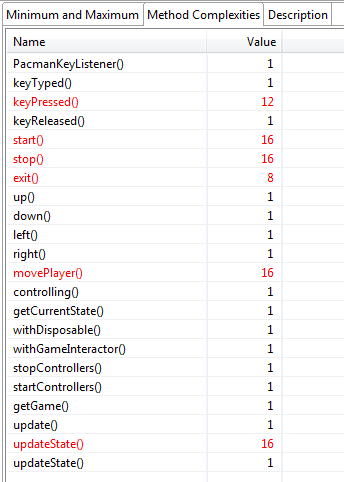
\includegraphics[width=\textwidth]{ACC_PacmanKeyListener.png}
	\caption{\label{ACC1}Détails de l'analyse de la complexité cyclique de la classe "PacmanKeyListener".}
\end{figure}
\begin{figure}[!h]
	\centering
	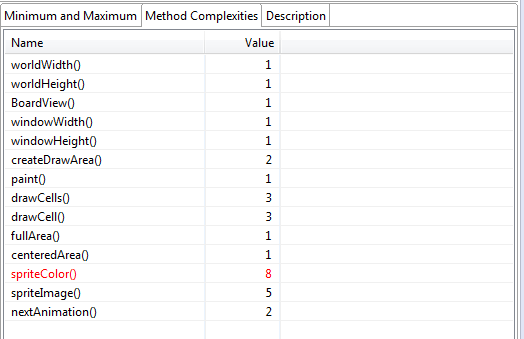
\includegraphics[width=\textwidth]{ACC_BoardView.png}
	\caption{\label{ACC2}Détails de l'analyse de la complexité cyclique de la classe "BoardView".}
\end{figure}
Pour chacun des cas illustrés dans la \labelfigure{ACC1} et la \labelfigure{ACC2}, il sera nécéssaire lors du refactoring (voir \ref{sec:etape3} ) d'analyser et de voir s'il sera possible de la diminuer.

\clearpage
\begin{figure}[!h]
	\centering
	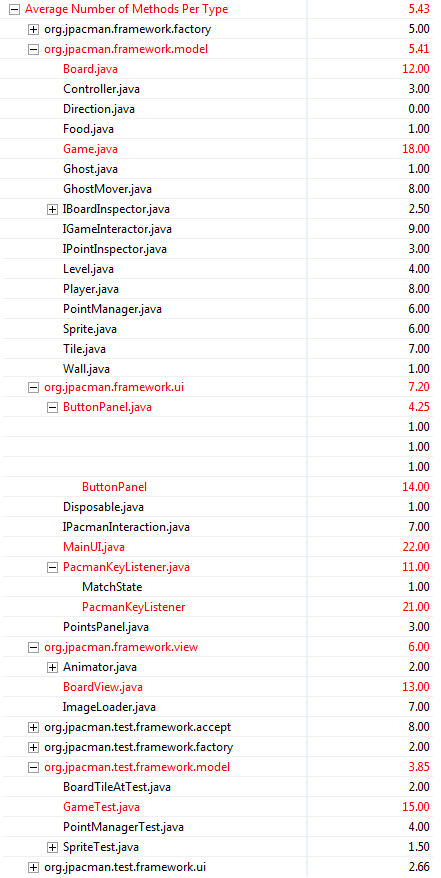
\includegraphics[height=\textheight]{Metrique1.png}
	\caption{\label{métrique1}Détails de l'analyse des métriques du projet (partie2).}
\end{figure}

\smalltitle{Nombre moyen de méthodes par type}
C'est la moyenne du nombre de méthodes définies pour chaque type défini dans les éléments cibles.
On remarque que certainnes classes ont trop de méthodes.
!!!!!!!!!!!!!!!!!!!!!!!!!!
\begin{figure}[!h]
	\centering
	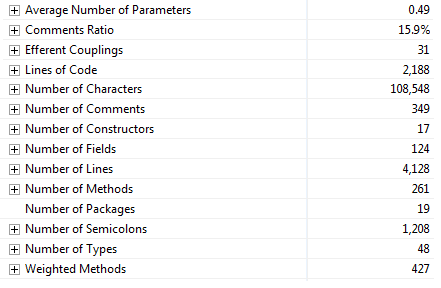
\includegraphics{Metrique2.png}
	\caption{\label{métrique2}Détails de l'analyse des métriques du projet (partie3).}
\end{figure}


\clearpage
\subsubsection{Audit}
Cet intitulé reprend tous les problèmes et les erreurs de code tel que les erreurs non capturées, la sérialisation les imports inutiles, les droit d'accès,...\\
Voici celles détectées par l'outil CodePro d'Eclipse : 
\begin{figure}[!h]
	\centering
	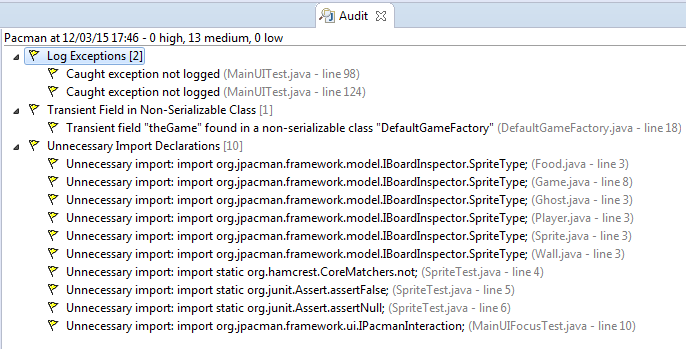
\includegraphics[width=\textwidth]{Audit.png}
	\caption{\label{Audit}Détail de l'analyse d'audit faite par Eclipse.}
\end{figure}

\smalltitle{Erreur non capturée}
Il s'agit de morceaux de code à risque (qui peuvent provoquer l'arrêt du programme avec une erreur fatale) qui n'est pas protégé.
Ici, les deux cas repéré sont encédré par un bloc "try...catch" mais ils ne capturent qu'un type d'exception. Pour résoudre ce problème il suffira d'ajouter un second bloc "catch" qui prenne en charge l'ensemble des autres exceptions.

\smalltitle{Sérialisation}
Un objet est sérialisable quand il implémente la classe "Serializable". Au sein d'un tel objet, tous les éléments doivent, par défaut, pouvoir l'être aussi. Dans le cas contraite, une variable globale peut-être qualifée avec le mot clé "`transient"` pour déclarer cette variable non sérialisable.
Dans ce cas-ci, l'objet DefaultGameFactory n'implémente pas la classe "Serializable" donc il n'y a aucune raison de déclarer une variable "transient".

\smalltitle{Import inutile}
Les imports sont les premières lignes d'une classe. Ils permettent d'informer au compilateur d'où viennent les méthodes, les objets,... utilisées qui ne sont pas créé au sein de la classe courante.
Egalement repris plus loin dans les warnings d'Eclipse, les classes comportent plusieurs imports qui ne sont jamais utilisé.
La meilleur solution est simplement de les supprimer.\\
Voici celles détectées par l'outil Code Inspector d'IntelijIdea : 
\begin{figure}[!h]
	\centering
	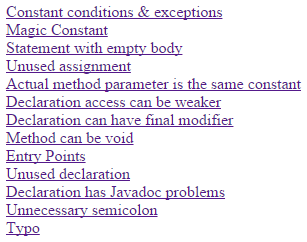
\includegraphics{AuditII.png}
	\caption{\label{Audit}Détail de l'analyse d'audit faite par IntelijIdea.}
\end{figure}

\smalltitle{Droit d'accès}
Chaque élément d'un code (classe, sous-classe, méthode, variable,...) est qualifié d'un mot-clé qui permet de définir l'accessibilité tel que (pour une variable globale ou une méthode\footnote{un descriptif similaire peut-être fait pour une classe}): 
\begin{itemize}
\item public : \\
- Est accessible dans la class\\
- Peut être accessible depuis une autre class du package ou elle se trouve.\\
- Peut être accessible depuis n'importe quelle class extérieur au package.
\item protected :\\
- Est accessible dans la class\\
- Peut-être accessible depuis une autre class du package ou elle se trouve (et des classes enfents).\\
- N'est pas accessible depuis n'importe quelle class extérieur au package.
\item private :\\
- est accessible dans la class\\
- Ne peut pas être accessible depuis une autre class du package ou elle se trouve.\\
- N'est pas accessible depuis n'importe quelle class extérieur au package.
\end{itemize}
Une mauvaise pratique est de tout mettre en publique. Ca permet une vue d'ensemble sur son programme mais implique parfois certaines erreurs d'utilisation.\\
Ce n'est donc pas un grave problème à l'heure actuelle puisque le jeux fonctionne correctement mais lors de l'ajout de fonctionnalité cela peut le devenir.

\smalltitle{Optimisation}
En java, une variable qui ne doit pas être modifié pendant le temps d'une exécution peut-être qualifiée avec le mot-clé "final". Ceci permet d'optimiser le code et de ne pas être confronté à une mauvaise utilisation de la variable par la suite.


\smalltitle{Restructuration}
Cet outil informe que la fonction "public int addPoints(int)" de la classe "org.jpacman.framework.model.Player" retourne une valeur qui n'est jamais utilisée et qui dont pourrait-être transformé en "public void addPoints(int)".\\
Cette modification est à étudier avant d'agir pour vérifier s'il n'est pas nécéssaire pour une utilisation postérieur de garder cette valeur de retour.\\
Il informe aussi que deux autres fonctions reçoivent toujours la même valeur dans leur paramètre et que donc cette valeur pourrait devenir une constante.\\
Chacun des cas sera à étudier pour savoir si cette information est disponible à la méthode et que celle-ci doit alors être refactorée ou si elle a été miseen paramètre en vue d'une améliorationfuture.

\smalltitle{Code inutile}
Ce sujet a déjà été traité plus haut (Voir \ref{deadCode}).


\smalltitle{Javadoc}
Ce sujet a déjà été traité plus haut (Voir \ref{javadoc}).


\smalltitle{Caractère inutile}
Ce sont des élément du code qui sont sous-entendu par le reste de l'architucture du code.\\
Dans ce projet, un seul cas a été resencé, il s'agit d'un ";" dans la classe "IBoardInspector" du package "org.jpacman.framework.model". Lors du refactoring, il suffira de le retirer.


\smalltitle{Typographie}
Les problèmes de typographies reprennent les erreurs de formatage des différents éléments. Ce ne sont des erreurs que de conventions parce que elle ne change en rien le comportement de l'application. Cependant, un bon respect des conventions permet une meilleur compréhension lors d'une relecture, d'une modification, de l'étude du code par un nouveau développeur sur le projet,...\\
L'outil Code Inspector intégré à IntelijIdea a permit d'en recenser plusieurs. A l'étude de celle-ci, il a été observé qu'elles sont souvent dans les commentaires. Exemple, dans le fichier "GhostMover.java" du package "org.jpacman.framework.model", entre la ligne 28 et la ligne 30, le mot "randomizer" a été identifié avec une majuscule dans le commentaire et sans majuscule dans les lignes de code.\\
\vspace{3cm}
Il est important de signaler aussi, que l'outil Eclipse soulève certaines attention à l'aide de "warnings".\\
Les types d'erreurs sont : 
\begin{itemize}
\item Empty block should be documented x2
\item Javadoc: Missing comment for public declaration x 51
\item Redundant specification of type arguments <...> x6
\item The import ... is never used x4
\item The method ... of type ... should be tagged with @Override since it actually overrides a superinterface method x13
\item The parameter ... is hiding a field from type ... x 7
\end {itemize}
Leurs emplacements : \\
\begin{tabular}{|l|l|l|l|}
\hline
Package & \# warning & Classe & \# warnings \\
\hline
/main/java/.../model & 60 & Game.java & 15 \\
&& IBoardInspector.java & 13 \\
&& Direction.java & 8 \\
&& Player.java & 7 \\
&& Board.java & 4 \\
&& IPointInspector.java & 3 \\
&& PointManager.java & 3 \\
&& Tile.java & 3 \\
&& GhostMover.java & 2 \\
&& Sprite.java & 1 \\
&& Food.java & 1 \\
\hline
/main/java/.../ui & 15 & ButtonPanel.java & 8 \\
&& PacmanKeyListener.java & 5 \\
&& MainUI.java & 2 \\
\hline
/test/java/.../model & 5 & SpriteTest.java & 5 \\
\hline
main/java/.../factory & 2 & MapParser.java & 2 \\
\hline
/test/java/.../ui & 1 & MainUIFocusTest.java & 1 \\
\hline
\end{tabular}

%%%%%%%%%%%%%%%%%%%%%%%%%%%%%%%%%%%%%%%%%%%%%%%%%%%%%%%%%%%%%%%%%%%%%%%%%%%%%%%%%%
\newpage
\section{Etape 2 : Ajout de tests unitaires}\label{sec:etape2}
\subsection{Enoncé}
Votre première analyse a révélé la présence de certains problèmes de qualité du code de l'application.
Avant d'envisager la correction de ces problèmes, il faut s'assurer que les modifications que vous apporterez au code source ne modifieront pas le comportement du logiciel.
Etendez et complétez le jeu de tests unitaires fourni avec le code source afin de vous prémunir d'une telle modification. Effectuez également une analyse de couverture de tests.
Quelle garantie avez-vous que vos futures modifications ne pourront pas casser le système ?

\subsection{Résultat}

Tests  Eclipse -> Coverage As -> JUnit Test : La figure \annexe{coverage} montre que le projet est couvert à $68.3 \%$ avec en particulier, $63.5\%$ pour la package \emph{main} et $83.7\%$ pour le package \emph{test}.
 Il est donc important d'ajouter des tests sur les classes : FactoryException, Board, Sprite et PacmanKeyListener qui sont sous le seuil des $50 \%$ de couverture.

%%%%%%%%%%%%%%%%%%%%%%%%%%%%%%%%%%%%%%%%%%%%%%%%%%%%%%%%%%%%%%%%%%%%%%%%%%%%%%%%%%
\newpage
\section{Etape 3 : Refactoring en vue d'améliorer la qualité}\label{sec:etape3}
\subsection{Enoncé}
Avec les tests unitaires ajoutés dans l'étape précédente, vous pouvez vérifier automatiquement (jusqu'à un certain point) la préservation du comportement du logiciel. Réalisez les modifications nécessaires à l'amélioration de la qualité et la structure du logiciel. 
Vos ressources et votre temps étant limités, commencez par établir les modifications devant être réalisées en priorité. Sur base de quels critères réalisez-vous cette priorisation ?
Refactorisez progressivement votre code, en vous assurant systématiquement que tous les tests déjà présents s'exécutent avec succès. Souvenez-vous que vos modifications doivent améliorer la qualité du code, et non étendre ou modifier le comportement du logiciel.

\subsection{Résultat}



%%%%%%%%%%%%%%%%%%%%%%%%%%%%%%%%%%%%%%%%%%%%%%%%%%%%%%%%%%%%%%%%%%%%%%%%%%%%%%%%%%
\newpage
\section{Etape 4 : Analyse de la qualité du logiciel}\label{sec:etape4}
\subsection{Enoncé}
Réalisez une étude similaire à celle décrite en Section ... La qualité du logiciel s'est-elle améliorée ? Les problèmes les plus critiques ont-ils été résolus ? Au vu de cette seconde analyse, quels sont les points qui devraient à présent être améliorés ?
\subsection{Résultat}



%%%%%%%%%%%%%%%%%%%%%%%%%%%%%%%%%%%%%%%%%%%%%%%%%%%%%%%%%%%%%%%%%%%%%%%%%%%%%%%%%%
\newpage
\section{Etape 5 : Extensions}\label{sec:etape5}
\subsection{Enoncé} 
Il vous est demandé d'étendre le logiciel afin d'y ajouter certaines fonctionnalités ou d'en améliorer la qualité. Chaque équipe doit réaliser au moins deux extensions diférentes, décrites dans la section ... .
Utilisez un processus de développement dirigé par les tests (test-driven development) : lors du développement des extensions, ajoutez de nouveaux tests unitaires pour tester le comportement prévu de l'extension. Effectuez également des tests de régression avec les tests unitaires déjà présents, afin de vous assurer que le comportement initial n'a pas été modifié.
\subsection{Résultat}



%%%%%%%%%%%%%%%%%%%%%%%%%%%%%%%%%%%%%%%%%%%%%%%%%%%%%%%%%%%%%%%%%%%%%%%%%%%%%%%%%%
\newpage
\section{Etape 6 : Analyse de la qualité du logiciel}\label{sec:etape6}
\subsection{Enoncé} 
Pour chaque extension ajoutée, réalisez une analyse de qualité similaire à celle décrite en Section ... Au vu de cette analyse, quels sont les points qui devraient à présent être améliorés ?
\subsection{Résultat}



%%%%%%%%%%%%%%%%%%%%%%%%%%%%%%%%%%%%%%%%%%%%%%%%%%%%%%%%%%%%%%%%%%%%%%%%%%%%%%%%%%
\newpage
\section{Etape 7 : Analyse de l'évolution de la qualité logicielle}\label{sec:etape7}
\subsection{Enoncé} 
Analysez l'évolution de la qualité du logiciel entre les diférentes versions, en utilisant les résultats d'analyse de qualité des sections ..., ... et ... . Montrez cette évolution graphiquement et interprètez-la.
\subsection{Résultat}

%%%%%%%%%%%%%%%%%%%%%%%%%%%%%%%%%%%%%%%%%%%%%%%%%%%%%%%%%%%%%%%%%%%%%%%%%%%%%%%%%%
\clearpage
\newpage
\section{Annexes} \label{sec:annexe}
\appendix %permet de changer la numérotation en lettre
\section{Annexe : Code Dupliqué}\label{SimilarCode}
Dans cette section se trouve les différentes annexes qui permettent d'identifier les blocs de code dupliqués détectés par CodePro. Chaque image illustre un bloc de code mis à part la dernière qui illustre les 6 derniers blocs de code et est issue du rapport généré par CodePro (parce que Eclipse les masque).
N.B. : La figure repprennant tous les blocs identifié se trouve à la sous-section \ref{codeduplique}

\begin{figure}[ht]
	\centering
	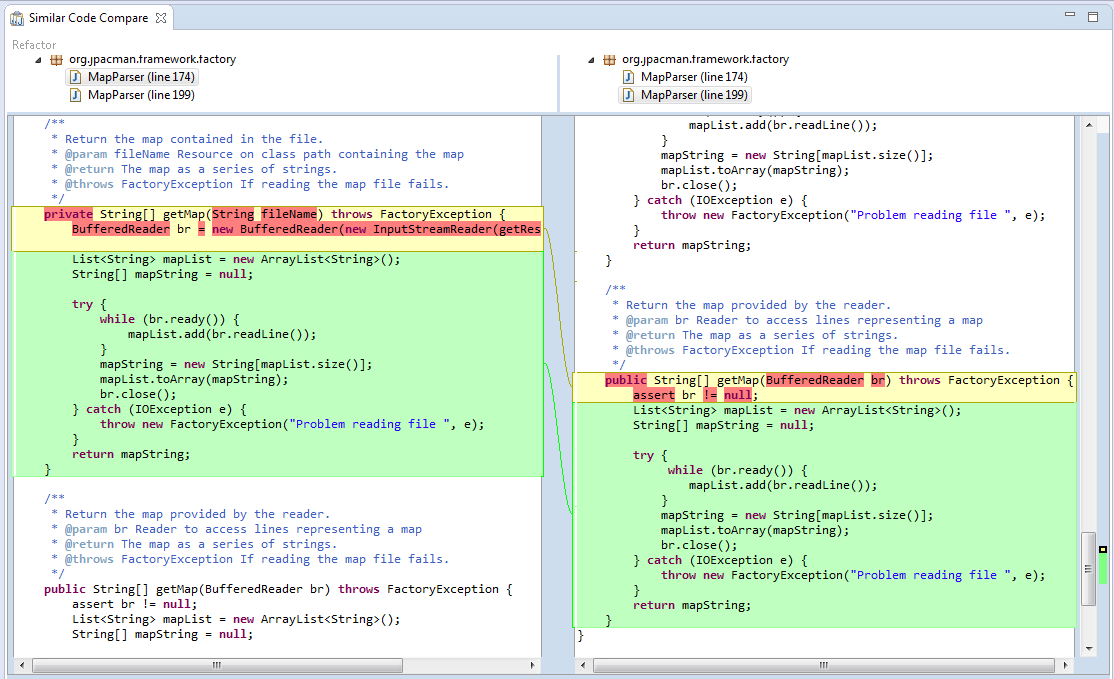
\includegraphics[width=\textwidth]{images/SimilarCode_1.png}
	\caption{\label{SimilarCode1}Détail de l'analyse de code redondant par CodePro}
\end{figure}

\begin{figure}[ht]
	\centering
	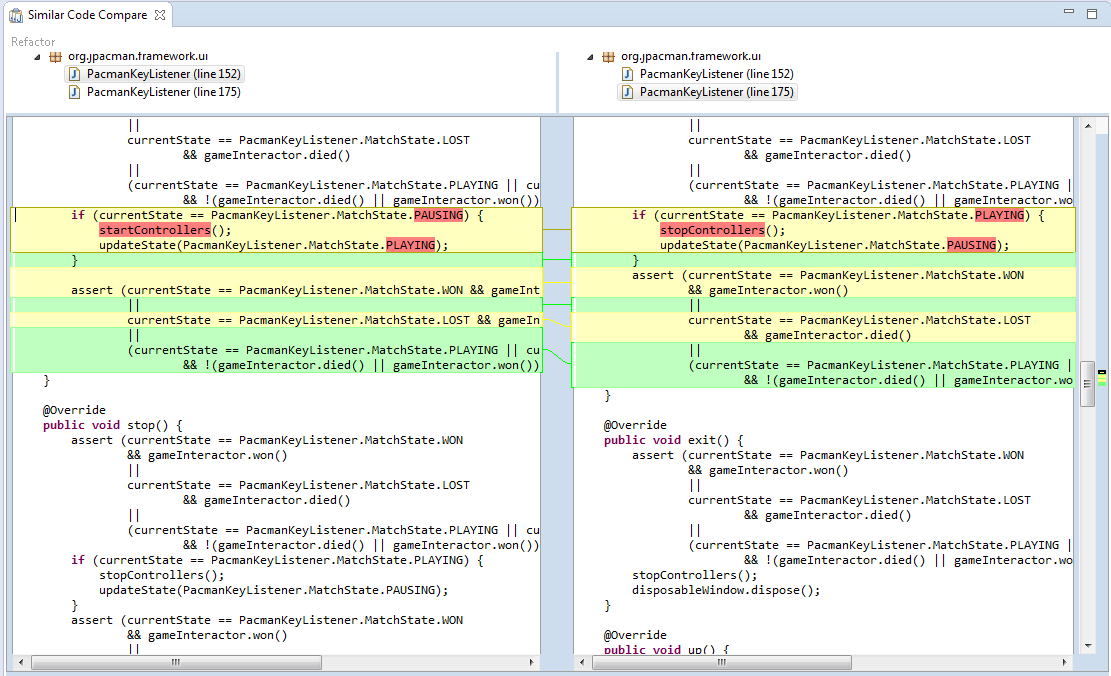
\includegraphics[width=\textwidth]{images/SimilarCode_2.png}
	\caption{\label{SimilarCode2}Détail de l'analyse de code redondant par CodePro}
\end{figure}

\begin{figure}[ht]
	\centering
	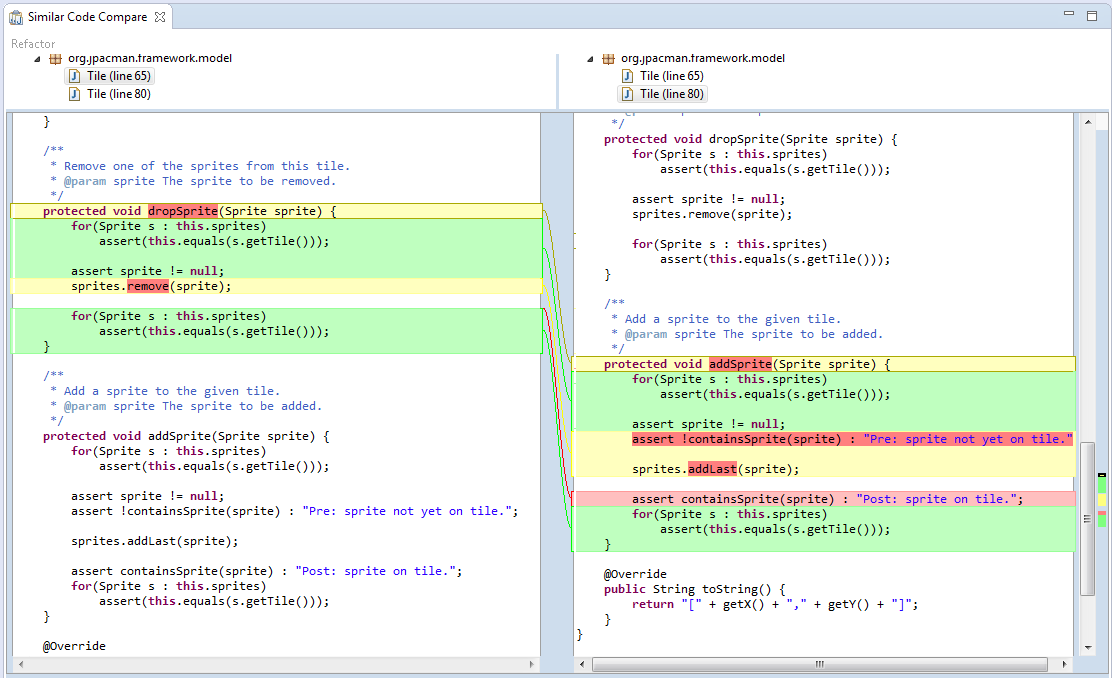
\includegraphics[width=\textwidth]{images/SimilarCode_3.png}
	\caption{\label{SimilarCode3}Détail de l'analyse de code redondant par CodePro}
\end{figure}

\begin{figure}[ht]
	\centering
	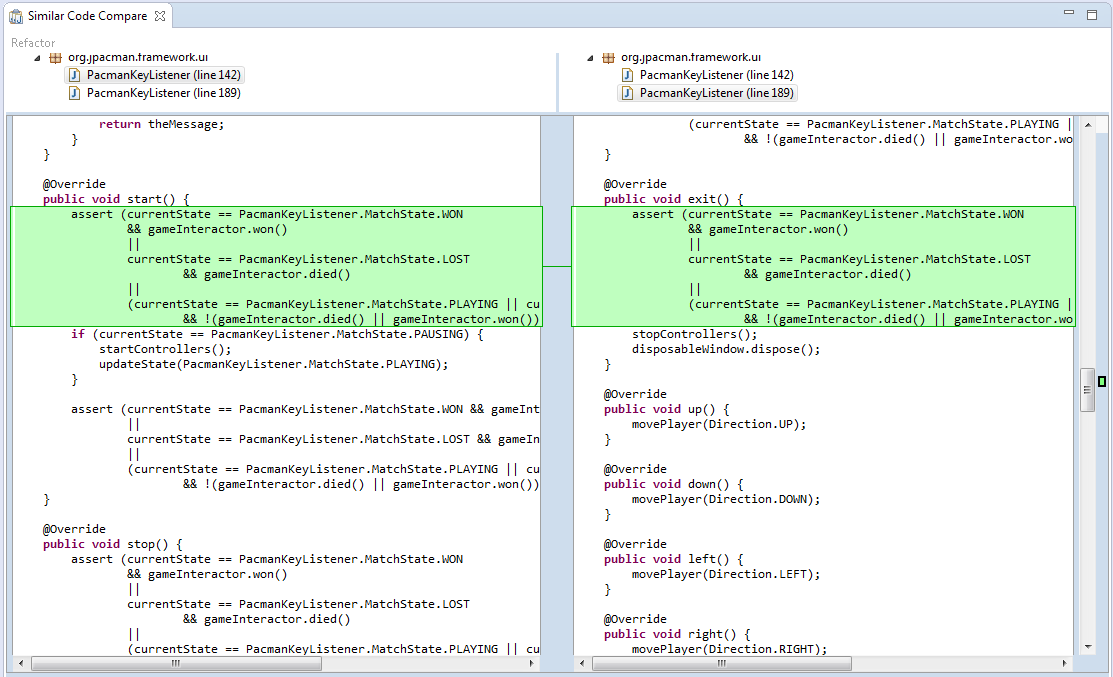
\includegraphics[width=\textwidth]{images/SimilarCode_4.png}
	\caption{\label{SimilarCode4}Détail de l'analyse de code redondant par CodePro}
\end{figure}

\begin{figure}[ht]
	\centering
	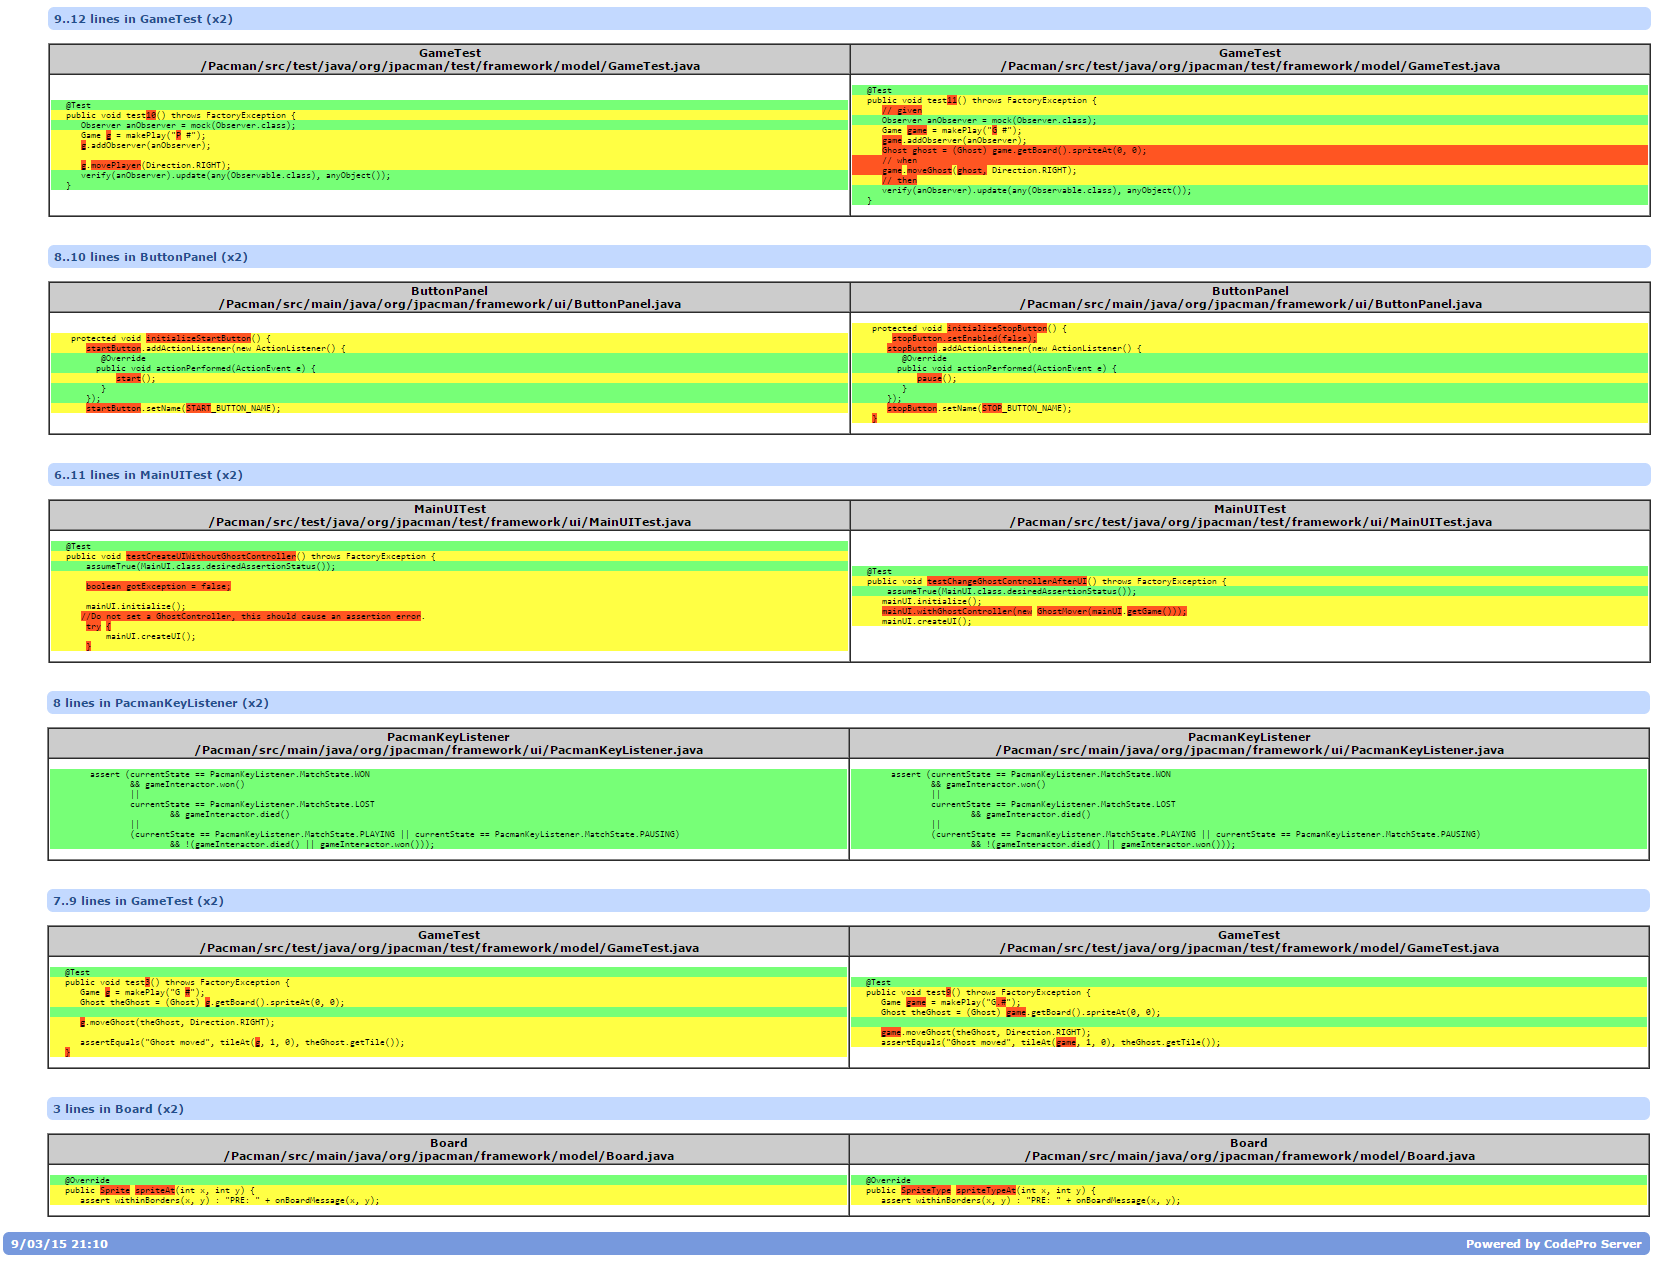
\includegraphics[width=\textwidth]{images/SimilarCode_5.png}
	\caption{\label{SimilarCode5}Détail de l'analyse de code redondant par CodePro (élément dont la visualisation n'est pas possible dans Eclipse)}
\end{figure}

\clearpage
\newpage
\section{Annexe : Dépendances}\label{Dependencies}
Ces figures permettent de visualiser les dépendances entre les différents éléments du projet.
N.B. : Les figures des dépendances entre les packages et des dépendances au sein du package Model se trouve  à la sous-section \ref{dépendances}.

\begin{figure}[ht]
	\centering
	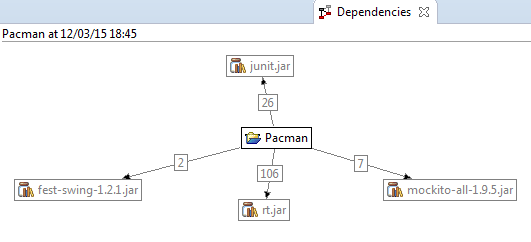
\includegraphics[width=\textwidth]{images/DependenciesProject.png}
	\caption{\label{dependenciesP}Détail de l'analyse des dépendences cycliques du projet.}
\end{figure}

\begin{figure}[ht]
	\centering
	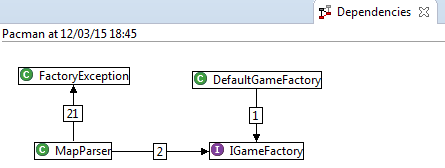
\includegraphics[width=\textwidth]{images/DependenciesFactory.png}
	\caption{\label{dependenciesF}Détail de l'analyse des dépendences cycliques du package Factory.}
\end{figure}

\begin{figure}[ht]
	\centering
	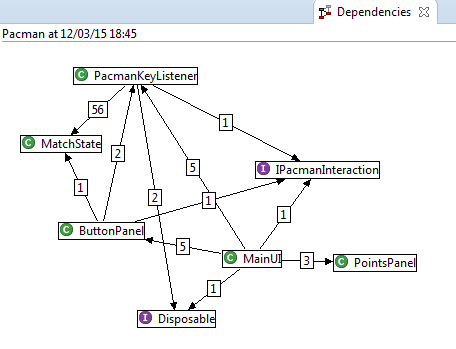
\includegraphics[width=\textwidth]{images/DependenciesUI.png}
	\caption{\label{dependenciesUI}Détail de l'analyse des dépendences cycliques du package UI.}
\end{figure}

\begin{figure}[ht]
	\centering
	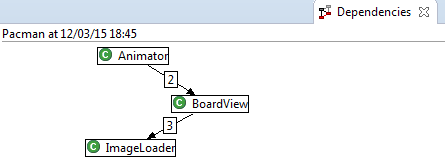
\includegraphics[width=\textwidth]{images/DependenciesVieuw.png}
	\caption{\label{dependenciesV}Détail de l'analyse des dépendences cycliques du package Vieuw.}
\end{figure}

\begin{figure}[ht]
	\centering
	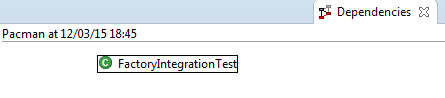
\includegraphics[width=\textwidth]{images/DependenciesFactoryTest.png}
	\caption{\label{dependenciesFT}Détail de l'analyse des dépendences cycliques du package Factory (Test).}
\end{figure}

\begin{figure}[ht]
	\centering
	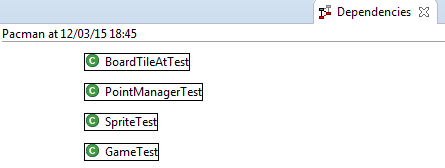
\includegraphics[width=\textwidth]{images/DependenciesModelTest.png}
	\caption{\label{dependenciesMT}Détail de l'analyse des dépendences cycliques du package Model (Test).}
\end{figure}

\begin{figure}[ht]
	\centering
	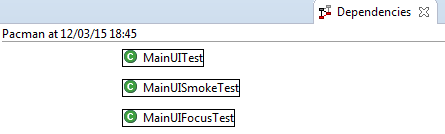
\includegraphics[width=\textwidth]{images/DependenciesUITest.png}
	\caption{\label{dependenciesUIT}Détail de l'analyse des dépendences cycliques du package UI (Test).}
\end{figure}

\begin{figure}[ht]
	\centering
	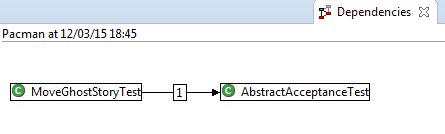
\includegraphics[width=\textwidth]{images/DependenciesAcceptTest.png}
	\caption{\label{dependenciesAT}Détail de l'analyse des dépendences cycliques du package Accept (Test).}
\end{figure}

\begin{figure}[ht]
	\centering
	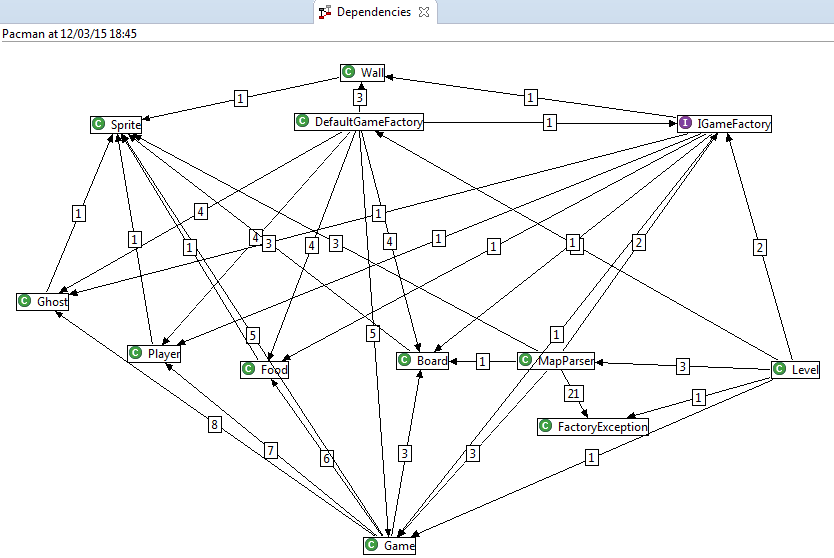
\includegraphics[width=\textwidth]{images/DependenciesModel_Factory.png} %images/DependenciesModel_Factory1.png
	\caption{\label{dependenciesMF}Détail de l'analyse des dépendences cycliques entre le package Model et la package Factory.} %avec en gras les classes du package Factory
\end{figure}


\clearpage
\newpage
\section{Annexe : Incode}\label{InCode}

\begin{figure}[ht]
	\centering
	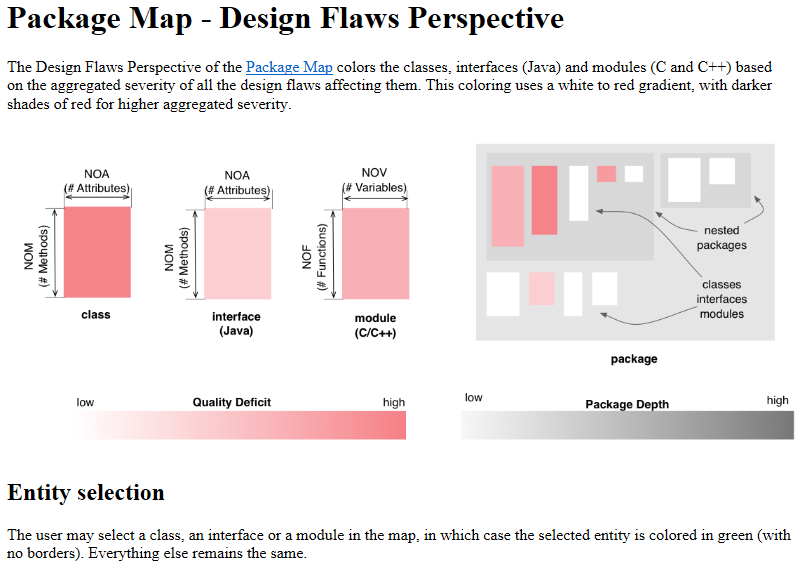
\includegraphics[width=\textwidth]{images/InCodeDesignFlawsLegende.png}
	\caption{\label{designflawsLeg}Légende de l'outil InCode d'analyse de conception}
\end{figure}

\begin{figure}[ht]
	\centering
	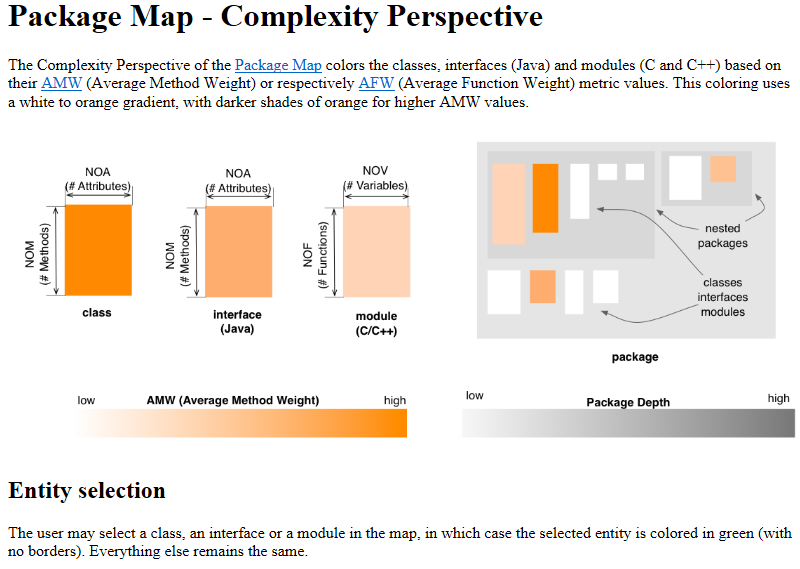
\includegraphics[width=\textwidth]{images/InCodeComplexityLegende.png}
	\caption{\label{complexityLeg}Légende de l'outil InCode d'analyse de complexité}
\end{figure}

\begin{figure}[ht]
	\centering
	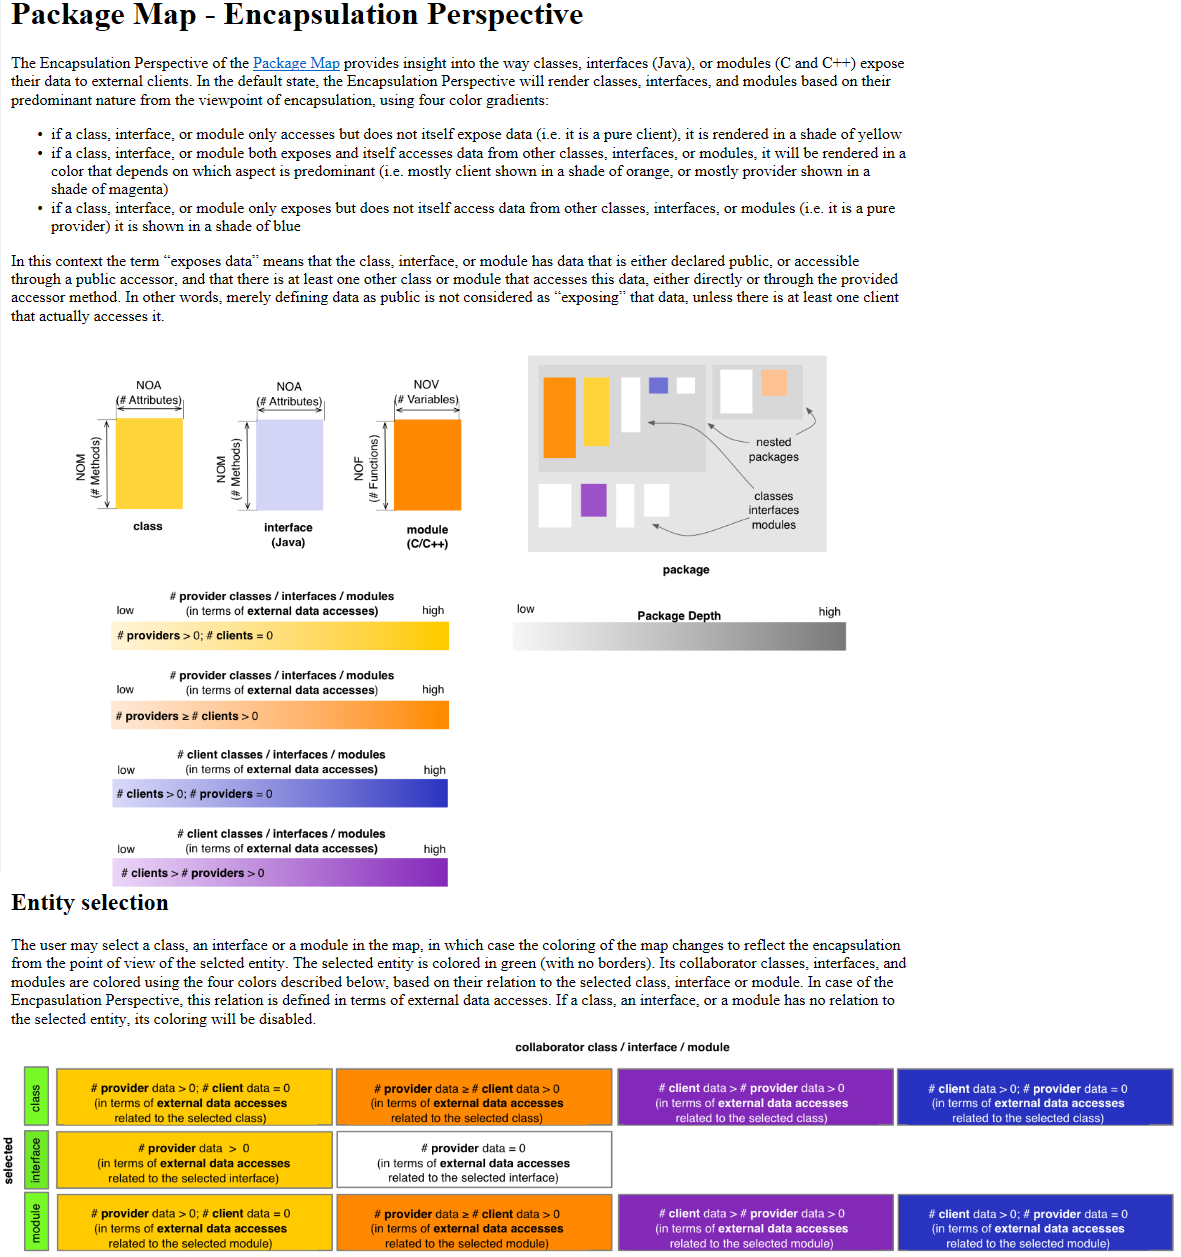
\includegraphics[width=\textwidth]{images/InCodeEncapsulationLegende.png}
	\caption{\label{encapsulationLeg}Légende de l'outil InCode d'analyse d'encapsulation}
\end{figure}

\begin{figure}[ht]
	\centering
	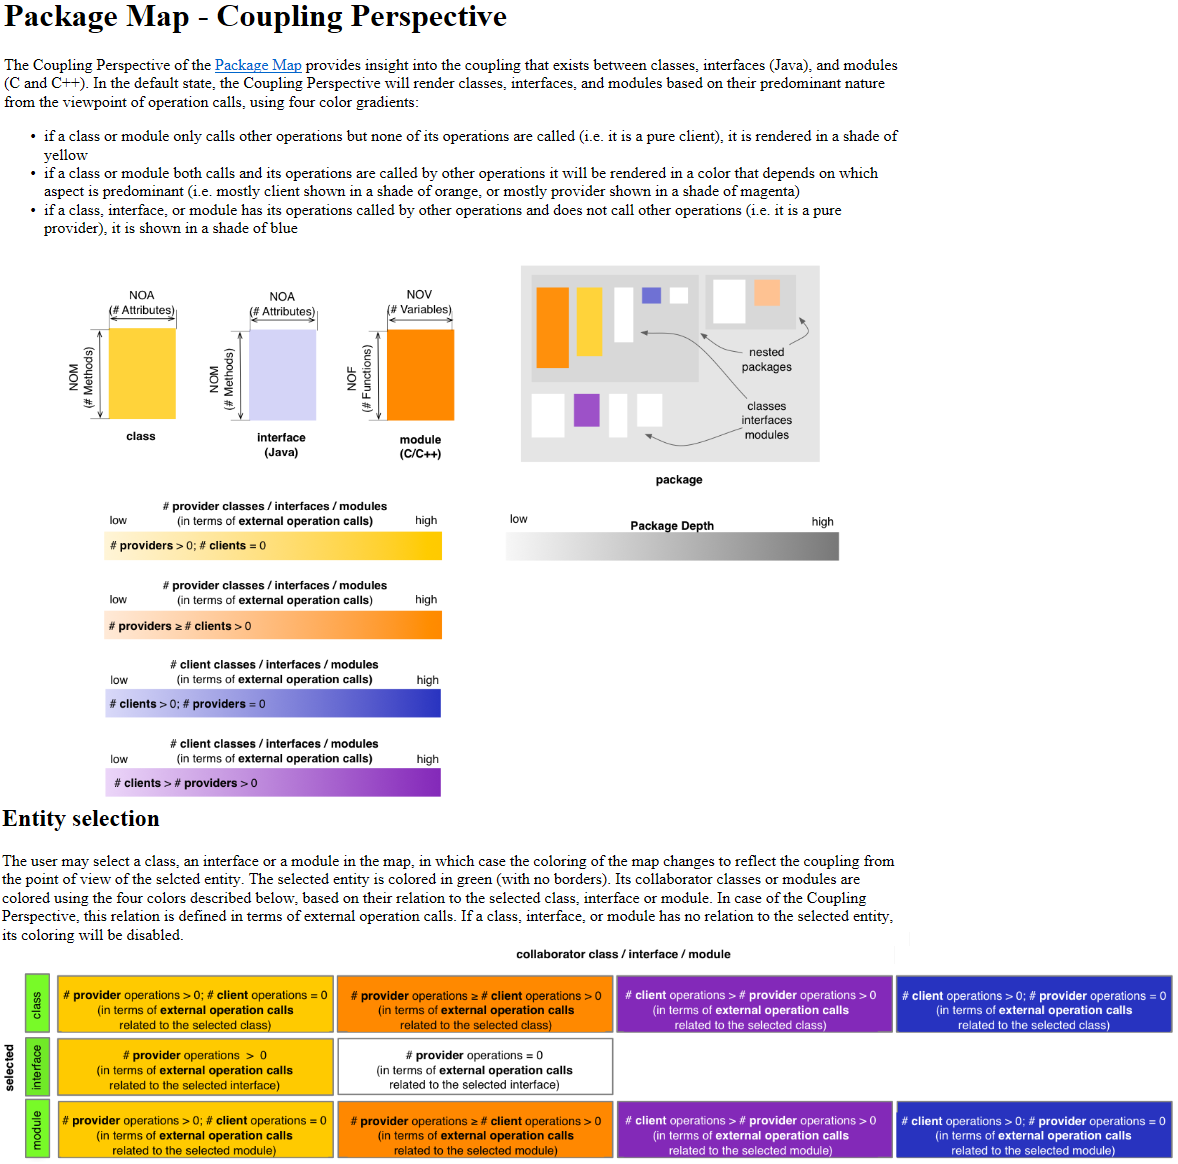
\includegraphics[width=\textwidth]{images/InCodeCouplingLegende.png}
	\caption{\label{couplingLeg}Légende de l'outil InCode d'analyse de couplage}
\end{figure}

\begin{figure}[ht]\label{pyramidLeg}
L'Aperçu Pyramide rassemble en un seul endroit les mesures les plus importantes sur un système orienté objet. Il se compose de trois parties, chacune quantifie un aspect important de la conception de systèmes orientés objet : la taille et la complexité, l'utilisation de l'héritage, et le couplage.

Le côté gauche de la pyramide aperçu (zone jaune) fournit des informations caractérisant la taille et la complexité du système. Ils comptent les unités les plus importantes de la modularité d'un système orienté objet, du plus haut niveau, jusqu'aux plus basses unités de mesures : 
• NOP (nombre total de packages définis dans le système);
• CNP ou NOC (nombre total de classes définies dans le système, sans compter les classes de la bibliothèque);
• NOM (nombre total de méthodes définies dans le système, y compris les méthodes et fonctions globales);
• LOC (nombre total de lignes de code appartenant à l'exploitation);
• CYCLO (somme des nombres cyclomatiques de toutes les opérations définies dans le système).
Les chiffres indiqués à la gauche de ces paramètres sont calculés par un rapport entre les mesures directement placés en dessous et à droite. où par exemple le rapport NOM / CNP représente le nombre moyen de méthodes dans une classe.

La partie supérieure de la pyramide (la zone verte) est dédié à l'utilisation de l'héritage : 
• NDD (nombre moyen de descendants directs d'une classe, à l'exclusion des classes de la bibliothèque. Si une classe n'a pas de classes dérivées, alors la classe participe avec une valeur de 0);
• HIT (moyenne de la métrique de HIT( = la longueur de trajet maximal d'une classe à sa plus profonde sous-classe) sur toutes les classes définies dans le système. Les classes autonomes sont considérés classes racines avec HIT = 0).

Le côté droit de la pyramide (la zone bleue) est dédié à l'aspect de couplage :
• CALL (nombre total d'opérations distinctes d'appelle dans le système);
• FOUT (somme de la métrique de FANOUT pour toutes les opérations définies dans le système)

Pour chaque rapport calculé, trois seuils sont calculés:
• faible - bleu
• Moyenne - vert
• haute - rouge
\end{figure}

\clearpage
\newpage
\section{Annexe : Couverture par les test}\label{coverage}

\begin{figure}[ht]
	\centering
	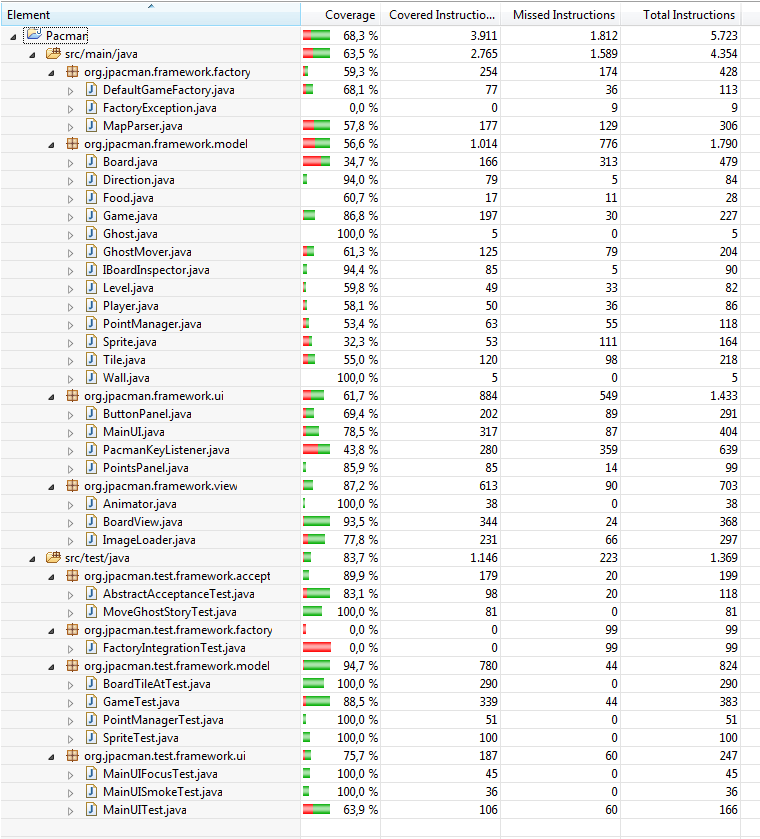
\includegraphics[width=\textwidth]{images/CoverageTest.png}
	\caption{\label{CoverageTest}Détail de l'analyse de couverture du code par les tests unitaires.}
\end{figure}





\newpage
\bibliographystyle{plain}
\bibliography{reference}

\end{document} 

